\documentclass[11pt]{article}
\usepackage[margin=1in]{geometry}
\usepackage{amsmath,amssymb,amsthm}
\usepackage[hidelinks]{hyperref}
\usepackage{graphicx}

\newtheorem{theorem}{Theorem}
\newtheorem{remark}{Remark}
\newtheorem{lemma}{Lemma}

\DeclareMathOperator{\spanop}{span}

\title{A Counterexample to the Initial-Segment Numerical-Index Problem}
\author{FA Banach run: \texttt{fa\_banach\_001}}
\date{2026-06-28}

\begin{document}
\maketitle

\section*{Source Problem}

The source paper is:
\begin{quote}
M. Martin, J. Meri, M. Popov, and B. Randrianantoanina,
\emph{Numerical index of absolute sums of Banach spaces},
arXiv:1003.3269.
\end{quote}

Problem 5.3 asks whether, if \(Z\) has a monotone basis
\((e_m)_{m\geq 1}\) and
\[
X_m=\spanop\{e_k:1\leq k\leq m\},
\]
then
\[
n(Z)=\limsup_{m\to\infty} n(X_m).
\]
The parenthetical version asks whether the assertion might remain true under
stronger hypotheses such as a one-unconditional, one-symmetric basis.

\begin{center}
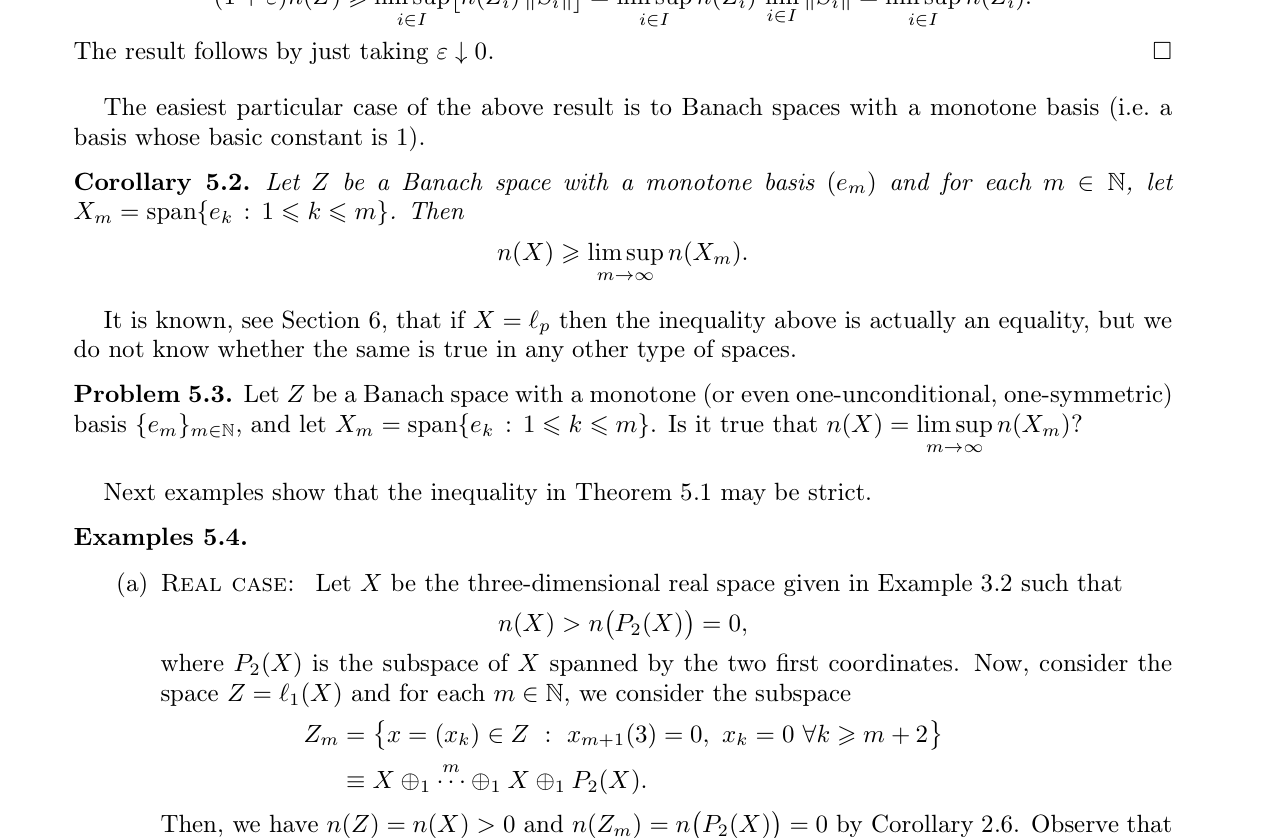
\includegraphics[width=0.92\textwidth]{figures/open_problem_and_source_example_crop.png}
\end{center}

\section*{Result}

\begin{theorem}
Problem 5.3 has a negative answer for monotone bases. In fact, there is a
real Banach space \(Z\) with a one-unconditional monotone basis
\((f_m)_{m\geq 1}\) such that, for
\[
F_m=\spanop\{f_1,\ldots,f_m\},
\]
one has
\[
n(Z)>0,\qquad n(F_m)=0\quad(m\geq 2).
\]
Consequently,
\[
n(Z)>\limsup_{m\to\infty} n(F_m).
\]
\end{theorem}

\section*{Proof Intuition}

The source paper already contains almost all of the construction. It gives a
three-dimensional real space \(X\) with a one-unconditional, one-symmetric
basis \((u,v,w)\), positive numerical index, and with
\(\spanop\{u,v\}\) isometric to the real Hilbert plane, hence numerical index
zero. The space \(Z=\ell_1(X)\) still has positive numerical index. The trick
is only to permute the natural basis of \(Z\): keep opening a new block before
closing the previous one. Then every sufficiently large initial segment has a
whole copy of the two-dimensional Hilbert plane as an \(\ell_1\)-summand, so
its numerical index is forced down to zero.

\section*{Proof}

Let \(X\) be the real three-dimensional space from Example 3.2 of the source
paper:
\[
\|(a,b,c)\|
=\max\left\{\sqrt{a^2+b^2},\sqrt{a^2+c^2},\sqrt{b^2+c^2}\right\}.
\]
The usual basis \((u,v,w)\) is one-unconditional and one-symmetric. The source
paper proves
\[
n(X)>0
\]
and observes that
\[
H:=\spanop\{u,v\}
\]
is isometric to the real two-dimensional Hilbert space. Hence \(n(H)=0\).

Set
\[
Z=\ell_1(X).
\]
For the \(j\)-th copy of \(X\), write its coordinate basis as
\[
u_j,\quad v_j,\quad w_j.
\]
By Corollary 2.6 of the source paper, the numerical index of an
\(\ell_1\)-sum is the infimum of the numerical indices of the summands, so
\[
n(Z)=n(\ell_1(X))=n(X)>0.
\]

Now order the coordinate vectors of \(Z\) as follows:
\[
f_1=u_1,\qquad f_2=v_1,
\]
and, for \(k\geq 1\),
\[
f_{3k}=u_{k+1},\qquad
f_{3k+1}=v_{k+1},\qquad
f_{3k+2}=w_k.
\]
Thus the sequence begins
\[
u_1,\ v_1,\ u_2,\ v_2,\ w_1,\ u_3,\ v_3,\ w_2,\ u_4,\ v_4,\ w_3,\ldots .
\]
This is a permutation of the natural one-unconditional basis of
\(\ell_1(X)\), hence it is again a one-unconditional monotone basis.

Fix \(m\geq 2\), and let
\[
F_m=\spanop\{f_1,\ldots,f_m\}.
\]
We claim that \(F_m\) contains, as an \(\ell_1\)-summand, a copy of
\[
H_j:=\spanop\{u_j,v_j\}
\]
for some \(j\), while \(w_j\notin F_m\). Indeed, after \(u_j\) and \(v_j\)
are listed, the vector \(w_j\) is not listed until after \(u_{j+1}\) and
\(v_{j+1}\). At every initial stage \(m\geq 2\), at least one currently open
block has exactly its first two coordinates present and its third coordinate
absent.

Since the norm on \(Z=\ell_1(X)\) is the sum of the block norms and the basis
of \(X\) is one-unconditional, each \(F_m\) is an \(\ell_1\)-sum of finitely
many coordinate subspaces of copies of \(X\). One of those summands is the
Hilbert plane \(H_j\), so Corollary 2.6 of the source paper gives
\[
n(F_m)=\min\{\text{numerical indices of the nonzero block summands of }F_m\}
\leq n(H_j)=0.
\]
As numerical indices are nonnegative, \(n(F_m)=0\) for every \(m\geq 2\).
Therefore
\[
\limsup_{m\to\infty} n(F_m)=0<n(Z),
\]
which disproves the asserted equality.
\qed

\section*{Complex Variant}

The same reordering also gives a complex one-unconditional counterexample,
although not with zero as the limiting value. Use Example 3.3 of the source
paper: a five-dimensional complex space \(X\) with one-unconditional basis,
\[
n(X)=1,
\]
and whose first four-coordinate subspace \(P_4(X)\) satisfies
\[
n(P_4(X))<1.
\]
In \(Z=\ell_1(X)\), list the first four coordinates of block \(j+1\) before
listing the fifth coordinate of block \(j\). Then every sufficiently large
initial segment has a \(P_4(X)\) summand, hence its numerical index is at most
\(n(P_4(X))<1\), while
\[
n(Z)=n(\ell_1(X))=n(X)=1.
\]
Thus the complex one-unconditional version is also false.

\section*{Limitations}

The construction uses a one-unconditional monotone basis, but the permutation
of coordinates destroys the global one-symmetry of the natural block basis.
It therefore does not settle the stronger one-symmetric variant mentioned in
Problem 5.3.

\section*{Novelty Check}

On 2026-06-28, I searched the web for exact and close variants of the problem:
\[
\texttt{"Numerical index of absolute sums of Banach spaces" "monotone" "basis" "limsup"},
\]
\[
\texttt{"n(X) = limsup" "numerical index" "monotone basis"},
\]
and
\[
\texttt{"numerical index" "dense increasing" "one-complemented subspaces"}.
\]
The only exact match found was the original arXiv paper. No later explicit
answer to Problem 5.3 was found in this bounded search.

\section*{References}

\begin{thebibliography}{9}
\bibitem{MMP-R}
M. Martin, J. Meri, M. Popov, and B. Randrianantoanina,
\emph{Numerical index of absolute sums of Banach spaces},
arXiv:1003.3269.
\end{thebibliography}

\end{document}
